
\section{Microgrid System Architecture}

The system under study is a grid-connected residential microgrid designed to minimize electricity costs through the intelligent management of energy storage. The architecture adopts an AC-coupled topology, where the photovoltaic (PV) generation, battery energy storage system (BESS), and residential loads are connected to a common AC bus at the Point of Common Coupling (PCC).

At any time step $t$, the power balance of the system is governed by Kirchhoff's Current Law, which necessitates that the algebraic sum of power flows at the PCC be zero. The relationship between the net grid power exchange ($P_{grid}$), residential load demand ($P_{load}$), PV generation ($P_{pv}$), and battery power ($P_{bat}$) is defined as:

\begin{equation}
    P_{grid}(t) = P_{load}(t) - P_{pv}(t) + P_{bat}(t)
\end{equation}

In this convention:
\begin{itemize}
    \item $P_{grid}(t) > 0$ denotes importing power from the utility grid (buying).
    \item $P_{grid}(t) < 0$ denotes exporting power to the utility grid (selling).
    \item $P_{bat}(t) > 0$ indicates charging the battery (consuming power from the bus).
    \item $P_{bat}(t) < 0$ indicates discharging the battery (supplying power to the bus).
\end{itemize}

The objective of the Energy Management System (EMS) is to control $P_{bat}(t)$ such that the total cost of electricity imported from the grid is minimized over a 24-hour horizon, subject to the operational constraints of the battery and the power limits of the grid connection. The system assumes a bidirectional power flow capability, allowing the prosumer to participate in energy arbitrage by buying low and selling high, provided that the net feed-in tariff structure supports such incentives.

\begin{figure}[ht]
    \centering
    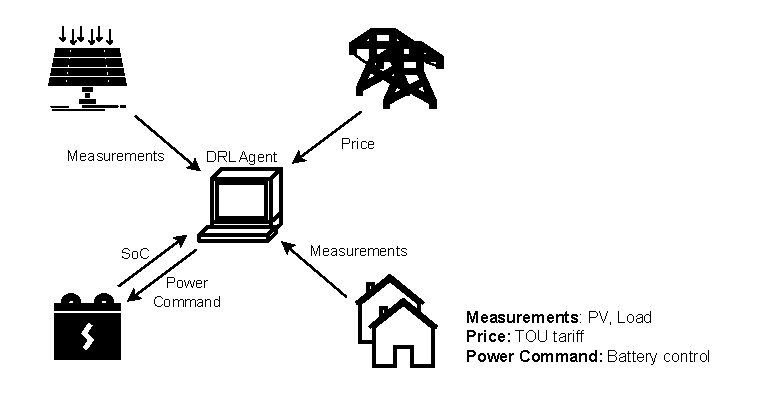
\includegraphics[width=1\textwidth]{Pages/fig/microgrid.pdf}
    \caption{Microgrid System Modeling}
    \label{fig:microgrid}
\end{figure}